\documentclass[12pt,a4paper]{article}

% ---------------------------------------------------------------------------------
% Fonts and layout
% ---------------------------------------------------------------------------------
\usepackage{amsmath}
\usepackage{txfonts}
\usepackage[no-math]{fontspec}
\setmainfont{TeX Gyre Termes}
\newfontfamily\appendixfont{Caladea}
\usepackage[a4paper,left=2.5cm,right=2.5cm,top=2.5cm,bottom=2.5cm,footskip=1.2cm]{geometry}
\usepackage{graphicx}
\usepackage{booktabs}
\usepackage{caption}
\captionsetup{labelsep=colon,justification=centering,font=normalsize,skip=6pt}
\usepackage{enumitem}
\usepackage{titlesec}
\usepackage[hang,flushmargin]{footmisc}
\usepackage[hidelinks,pdfauthor={David Duemig},pdftitle={Generating normally distributed pseudo-random numbers},pdfsubject={},pdfkeywords={},pdfcreator={},pdfproducer={}]{hyperref}

\setlength{\parindent}{0pt}
\setlength{\parskip}{6pt plus 1pt}
\setlength{\footnotesep}{10pt}
\renewcommand{\footnoterule}{\vspace*{-3pt}\noindent\rule{5cm}{0.4pt}\vspace*{2.6pt}}
\renewcommand{\arraystretch}{1.15}
\renewcommand{\floatpagefraction}{0.75}
\renewcommand{\topfraction}{0.85}
\renewcommand{\bottomfraction}{0.6}
\renewcommand{\textfraction}{0.1}

\titleformat{\section}{\fontsize{16}{19}\selectfont\bfseries}{\thesection}{1.2em}{}
\titlespacing*{\section}{0pt}{16pt}{4pt}
\titleformat{\subsection}{\fontsize{14}{17}\selectfont\bfseries}{\thesubsection}{0.9em}{}
\titlespacing*{\subsection}{0pt}{12pt}{2pt}
\titleformat{\subsubsection}{\normalsize\bfseries}{\thesubsubsection}{0.6em}{}
\titlespacing*{\subsubsection}{0pt}{10pt}{0pt}

\setlist[itemize]{label=\raisebox{0.2ex}{\scriptsize$\blacksquare$},leftmargin=1.4em,itemsep=4pt,topsep=2pt}
\setlist[enumerate]{leftmargin=1.8em,itemsep=0pt,topsep=2pt}
\newcommand{\head}[1]{\textbf{#1}\\}

% Generated by scripts/build_report.py from results/. Do not edit by hand.
\newcommand{\SampleSize}{5{,}000}
\newcommand{\Reps}{1{,}000}
\newcommand{\RateSE}{0.7}
\newcommand{\RateMin}{3.6\%}
\newcommand{\RateMax}{6.3\%}
\newcommand{\RateMaxZ}{2.0}
\newcommand{\TailDraws}{$10^{8}$}
\newcommand{\TailExpFour}{6{,}334}
\newcommand{\TailExpFive}{57.3}
\newcommand{\TailMinP}{0.07}
\newcommand{\TailMaxAbsZ}{0.8}
\newcommand{\InvMaxRel}{$1.2\times 10^{-15}$}
\newcommand{\AccRej}{0.760}
\newcommand{\AccRejTheory}{0.760}
\newcommand{\AccPolar}{0.785}
\newcommand{\AccPolarTheory}{0.785}
\newcommand{\UniPerDrawRej}{3.95}
\newcommand{\UniPerDrawPolar}{1.27}
\newcommand{\SpeedNumpy}{86}
\newcommand{\SpeedPolarLCG}{42}
\newcommand{\SpeedInvLCG}{21}
\newcommand{\CPU}{Intel Xeon Processor at 2.10GHz}
\newcommand{\UniPKS}{0.73}
\newcommand{\UniPChi}{0.95}
\newcommand{\UniPPairs}{0.74}
\newcommand{\VaRSheet}{78{,}329}
\newcommand{\ESSheetReported}{80{,}959}
\newcommand{\VaRSDPct}{7}
\newcommand{\ESSheet}{85{,}175}
\newcommand{\VaRRef}{79{,}166}
\newcommand{\ESRef}{90{,}413}
\newcommand{\VaRDN}{79{,}689}
\newcommand{\ESDN}{91{,}165}
\newcommand{\RefDraws}{10 million}
\newcommand{\VaRRankSheet}{56}
\newcommand{\ConvReps}{500}
\newcommand{\VaRSDFiveHundred}{5{,}458}
\newcommand{\VaRMeanFiveHundred}{78{,}052}
\newcommand{\VaRLoFiveHundred}{69{,}936}
\newcommand{\VaRHiFiveHundred}{87{,}738}
\newcommand{\ESLoFiveHundred}{79{,}328}
\newcommand{\ESHiFiveHundred}{100{,}870}
\newcommand{\VaRSDHundredK}{372}
\newcommand{\VaRSDTenK}{1{,}221}
\newcommand{\VaRBiasPct}{1.4}


\begin{document}

% ---------------------------------------------------------------------------------
% Title
% ---------------------------------------------------------------------------------
\thispagestyle{empty}
\vspace*{1.2cm}
\begin{center}
\rule{\textwidth}{3pt}\\[2pt]
{\fontsize{20}{24}\selectfont\bfseries Generating normally distributed\\ pseudo-random numbers\par}
\vspace{2pt}
\rule{\textwidth}{1.5pt}\\[14pt]
{\bfseries David Duemig}
\end{center}

\vspace{2.2cm}
\begin{center}
{\fontsize{16}{19}\selectfont\bfseries Abstract}
\end{center}
\vspace{-6pt}
\begin{list}{}{\leftmargin=1.9cm\rightmargin=1.9cm}\item[]
In this report, we examine four methods for generating pseudo-random numbers that follow the Gaussian (normal) distribution, starting from a simple uniform random number generator: inverse transform sampling, rejection sampling, the Box-Muller transformation and Marsaglia's polar method. To check whether what we have generated is actually Gaussian, we apply graphical methods and five statistical tests, both to single samples and to \Reps{} repeated samples, and we count extreme values in \TailDraws{} draws per method. We also compare the speed of the methods. Finally, to illustrate their application, we perform a Monte Carlo simulation in which we calculate the one-day Value-at-Risk (VaR) and Expected Shortfall (ES) of a portfolio of two ETFs, and we show how much the estimates depend on the number of simulated scenarios.
\end{list}

\vspace{1.2cm}
% ---------------------------------------------------------------------------------
\section{Introduction}

We often want to generate random draws from a certain probability distribution in the course of writing code for data analysis or for simulating the dynamics of the stock market. The problem is that most programming languages are only equipped with simple random number generators that generate uniformly distributed numbers between 0 and RAND\_MAX, where RAND\_MAX depends on the implementation and the language. The uniform distribution is sufficient when we need to simulate something simple, like rolling dice, but it is inadequate when other distributions are needed, such as the Gaussian, the Poisson or more exotic ones like the Gumbel distribution.

This report describes four different methods for generating numbers that are distributed with the Gaussian (normal) distribution, based on a simple uniform random number generator of the kind used in the C function \texttt{rand()}.\footnote{The code for this report, which produces every number, table and figure in it, can be found in the GitHub repository listed at the end.}

For comparison, we also generate samples with NumPy's default generator, which combines the PCG64 uniform generator (O'Neill, 2014) with the ziggurat method for normal draws (Marsaglia and Tsang, 2000).

In order to quantify the probability that what we have generated comes from a normal distribution, several normality tests are introduced. Because a single p-value says little about a generator, we also repeat every test on \Reps{} independent samples and check how often it rejects.

Finally, to illustrate the applications of our methods, we perform a Monte Carlo simulation to calculate the Value at Risk and Expected Shortfall of a portfolio consisting of ETFs on the S\&P 500 and the FTSE 100.

% ---------------------------------------------------------------------------------
\section{Methods}

In this section, we first describe the uniform generator and then present four different approaches to sample from a normal distribution.

\subsection{Uniform Pseudo-Random Numbers}

All four methods start from uniform random numbers on $(0,1)$. We generate them with a linear congruential generator (LCG),
\[
z_{i+1} = (a z_i + c) \bmod m, \qquad u_{i+1} = \frac{z_{i+1} + 0.5}{m},
\]
with $a = 1103515245$, $c = 12345$ and $m = 2^{32}$, the constants of the example \texttt{rand()} function in the ANSI C standard. Adding 0.5 keeps $u$ strictly between 0 and 1, so that $\ln(u)$ and the inverse normal CDF are always finite.

By the Hull-Dobell theorem (Hull and Dobell, 1962), an LCG has the full period $m$ for every seed if and only if (i) $c$ and $m$ are relatively prime, (ii) $a-1$ is divisible by all prime factors of $m$, and (iii) $a-1$ is a multiple of 4 if $m$ is a multiple of 4. All three conditions hold here ($c$ is odd and $a - 1 = 4 \times 275878811$), so the period is $2^{32} \approx 4.3 \times 10^{9}$.

An LCG with a power-of-two modulus has a known weakness in its low-order bits. Since $a$ and $c$ are odd, $z_{i+1} \equiv z_i + 1 \pmod 2$, so the last bit of $z$ simply alternates between 0 and 1. Dividing by $m$ moves these bits to the last digits of $u$, where they do no harm here, but they rule out using $z_i \bmod k$ directly for small $k$.

The recurrence is sequential, which makes it slow in an interpreted language when it is evaluated one step at a time. It can, however, be evaluated in blocks: for $k = 1, \dots, B$,
\[
z_{i+k} = (A_k z_i + C_k) \bmod m, \qquad A_k = a^k \bmod m, \qquad C_k = c\,(a^{k-1} + \dots + a + 1) \bmod m,
\]
so that a block of $B$ numbers is a single vectorised multiplication and addition. The output is identical to the step-by-step recurrence. Since $A_k$, $C_k$ and $z_i$ are smaller than $2^{32}$, $A_k z_i + C_k$ fits into an unsigned 64-bit integer.

\subsection{Inverse Transformation Sampling}

The inverse sampling algorithm allows us to generate random samples from a given probability distribution by using random samples from the uniform distribution and the cumulative distribution function (CDF) of the given distribution. The algorithm can be divided into two cases:

\begin{itemize}
\item \head{Case 1: CDF is invertible}
Let $F:\mathbb{R}\to(0,1)$ be an invertible CDF, i.e.\ there is $F^{-1}:(0,1)\to\mathbb{R}$ with $F^{-1}(F(x)) = x$ for all $x \in \mathbb{R}$ and $F(F^{-1}(a)) = a$ for all $a \in (0,1)$. Then, if $U \sim \text{Uniform}(0,1)$, $F^{-1}(U) \sim F$, i.e.\ $F^{-1}(U)$ has CDF $F$.
\item \head{Case 2: General case}
Let $F:\mathbb{R}\to(0,1)$ be a CDF and define $G:(0,1)\to\mathbb{R}$ by $G(a) = \inf\{x \in \mathbb{R}: a \le F(x)\}$. Then, if $U \sim \text{Uniform}(0,1)$, $G(U)$ has CDF $F$.
\end{itemize}

The proof for both cases can be found in the appendix.

Let $X$ be a random variable with distribution $N(\mu,\sigma^2)$. The PDF of $X$ is
\[
f_X(x) = \frac{1}{\sqrt{2\pi}\,\sigma}\exp\left(-\frac{(x-\mu)^2}{2\sigma^2}\right).
\]
The CDF is given by
\[
F(x) = P(X \le x) = \int_{-\infty}^{x}\frac{1}{\sqrt{2\pi}\,\sigma}\exp\left(-\frac{(t-\mu)^2}{2\sigma^2}\right)dt.
\]
The CDF of $N(\mu,\sigma^2)$ is a one-to-one and onto function from $\mathbb{R}$ to $(0,1)$. Thus, $F$ is invertible, and we can apply case 1. Since $X = \mu + \sigma Z$ with $Z \sim N(0,1)$, it is sufficient to invert the standard normal CDF $\Phi$ and set $X = \mu + \sigma\,\Phi^{-1}(U)$.

There is no closed-form expression for $\Phi^{-1}$, so it has to be approximated. We use Algorithm AS 241 of Wichura (1988), which approximates $\Phi^{-1}$ by three rational functions. For $|p - 0.5| \le 0.425$ it uses $\Phi^{-1}(p) = q\,A(r)/B(r)$ with $q = p - 0.5$ and $r = 0.180625 - q^2$, where $A$ and $B$ are polynomials of degree 7. In the tails it uses $r = \sqrt{-\ln(\min(p, 1-p))}$ and two further ratios of degree-7 polynomials, one for $r \le 5$ and one for $r > 5$. Section~\ref{sec:accuracy} checks the accuracy of our implementation.

\subsection{Rejection Sampling}

It is not always possible to find an explicit formula for the CDF of a random variable $X$ we want to generate samples for, or for its inverse. Furthermore, there may be alternative methods for generating samples with a distribution $F$ that are more efficient than the inverse transformation method.

In this section, we present a method known as the acceptance-rejection method. We assume that the distribution from which we want to sample has a probability density function $f(x)$. The basic idea is to find an alternative probability distribution with density function $g(x)$, for which we already have an efficient algorithm to generate samples (e.g., the inverse transform method). The function $g(x)$ should be ``close'' to $f(x)$; more specifically, we assume that the ratio $f(x)/g(x)$ is bounded by a constant $c > 0$, $\sup_x \{f(x)/g(x)\} \le c$. The complete algorithm and a proof can be found in the appendix.

If we want to generate samples for the random variable $X$, distributed as $N(\mu,\sigma^2)$, let $X = \sigma Z + \mu$, where $Z$ denotes a random variable with distribution $N(0,1)$. It is therefore sufficient to find an algorithm for generating $Z \sim N(0,1)$. Moreover, if we can generate from the absolute value $|Z|$, then by symmetry $Z$ can be obtained by independently generating a random variable $S$ (for sign) that is $\pm 1$ with probability 0.5 and setting $Z = S|Z|$. In other words, we generate $U$ and set $Z = |Z|$ if $U \le 0.5$ and $Z = -|Z|$ if $U > 0.5$.

$|Z|$ is non-negative and has the density
\[
f(x) = \frac{2}{\sqrt{2\pi}}\exp\left(-\frac{x^2}{2}\right), \qquad x \ge 0.
\]
For our alternative, we choose $g(x) = e^{-x}$, $x \ge 0$, the exponential density with rate 1, which we can sample with the inverse transform method. Noting that $h(x) = f(x)/g(x) = e^{x - x^2/2}\sqrt{2/\pi}$, we calculate its maximum by solving $h'(x) = 0$; it must occur at the value of $x$ that maximises the exponent.\footnote{The exponent $x - x^2/2$ is maximised at $x = 1$.} Therefore,
\[
c = \sqrt{2e/\pi} \approx 1.32, \qquad \text{and so} \qquad \frac{f(y)}{c\,g(y)} = e^{-(y-1)^2/2}.
\]
Accordingly, the algorithm for generating $Z$ looks as follows:
\begin{enumerate}
\item Generate $Y$ with an exponential distribution with rate 1, i.e.\ generate $U$ and set $Y = -\ln(U)$.
\item Generate $U$.
\item If $U \le e^{-(Y-1)^2/2}$, set $|Z| = Y$; otherwise go back to 1.
\item Generate $U$. Set $Z = |Z|$ if $U \le 0.5$ and $Z = -|Z|$ if $U > 0.5$.
\end{enumerate}
A proposal is accepted with probability $1/c \approx 0.760$ (see the appendix). Our implementation uses three uniforms per proposal, so it needs on average $3c \approx \UniPerDrawRej$ uniforms per normal draw. It is vectorised by generating a batch of proposals at once, keeping the accepted ones and repeating until enough values are available.

\subsection{Box-Muller Transformation}

The Box-Muller transformation (Box and Muller, 1958) uses uniform random deviates to generate $Z \sim N(0,1)$. Suppose $u_1$ and $u_2$ are independent random variables that are uniformly distributed on $(0,1)$ and let
\[
z_1 = \sqrt{-2\ln(u_1)}\,\cos(2\pi u_2), \qquad z_2 = \sqrt{-2\ln(u_1)}\,\sin(2\pi u_2).
\]
Then $z_1$ and $z_2$ are independent random variables with a standard normal distribution. The proof can be found in the appendix. To directly generate $X \sim N(\mu,\sigma^2)$ (Murison, 2000), we set $x = z\sigma + \mu$ and obtain
\[
x_1 = \sqrt{-2\ln(u_1)}\,\cos(2\pi u_2)\,\sigma + \mu, \qquad x_2 = \sqrt{-2\ln(u_1)}\,\sin(2\pi u_2)\,\sigma + \mu.
\]
Each pair of uniforms gives two normal draws, so the method needs exactly one uniform per draw and involves no rejection. Its cost lies in the logarithm, the square root and the two trigonometric functions.

\subsection{Marsaglia's Polar Method}

The polar method of Marsaglia and Bray (1964) avoids the sine and cosine. Let $V_1$ and $V_2$ be independent and uniform on $(-1,1)$, and $S = V_1^2 + V_2^2$. If $S \ge 1$ or $S = 0$, the pair is rejected and a new one is drawn. Otherwise, $(V_1, V_2)$ is uniform on the unit disc, $S$ is uniform on $(0,1)$ and independent of the angle $\theta$ of the point, and $(V_1, V_2)/\sqrt{S} = (\cos\theta, \sin\theta)$. Hence
\[
z_1 = V_1\sqrt{\frac{-2\ln S}{S}}, \qquad z_2 = V_2\sqrt{\frac{-2\ln S}{S}}
\]
are the Box-Muller pair with $u_1 = S$ and $2\pi u_2 = \theta$, and thus independent standard normal random variables. A pair is accepted with probability $\pi/4 \approx 0.785$, so the method uses on average $4/\pi \approx \UniPerDrawPolar$ uniforms per normal draw.

% ---------------------------------------------------------------------------------
\section{Normality Tests}

There are a number of techniques to determine whether what we have generated is Gaussian. In this report, we look at two types of techniques to check whether a data sample is normally distributed, and at a few tests of the uniform generator itself.

\subsection{Graphical Methods}

These are methods for displaying the data and for qualitatively evaluating whether the data sample looks Gaussian. Figures~\ref{fig:hist} and~\ref{fig:qq} show histograms, Q-Q plots and box plots of our samples.

\begin{itemize}
\item \head{Histogram}
One simple and frequently used graphical representation to check whether our data sample is normally distributed is the histogram. A Gaussian distribution is indicated when the histogram shows the well-known bell shape.
\item \head{Box Plot}
If our data sample is drawn from a Gaussian distribution, the box will be symmetrical with the mean and median in the centre. Moreover, if the data sample corresponds to the assumption of normality, we should observe only a few outliers.
\item \head{Probability-Probability Plot}
The probability-probability plot, or P-P plot for short, is a probability plot that can be used to assess how closely our data sample agrees with the normal distribution. A P-P plot is a scatterplot created by plotting the probabilities of the sample distribution and the probabilities of the theoretical distribution against each other. The resulting points are displayed with the theoretical value on the x-axis and the data sample on the y-axis. If both came from the same distribution, we should observe a line of points at an angle of 45 degrees from the bottom left to the top right.
\item \head{Quantile-Quantile Plot}
The quantile-quantile plot, or Q-Q plot for short, is similar to the P-P plot and is another graphical method we use to determine whether our data sample comes from the normal distribution. A Q-Q plot is a scatterplot created by plotting the quantiles of the sample distribution and the quantiles of the theoretical distribution against each other. If both sets of quantiles came from the same distribution, we should again observe a line of points at an angle of 45 degrees. Unlike the P-P plot, the Q-Q plot shows deviations in the tails clearly.
\item \head{Empirical CDF Plot}
An empirical CDF plot has a similar function to a P-P plot. However, unlike a probability plot, the empirical CDF plot has scales that are not transformed, and the fitted distribution does not form a straight line, but an S-shaped curve under normality. The empirical cumulative probabilities should lie close to this S-shaped curve.
\end{itemize}

\subsection{Statistical Tests}

These are methods to quantify the evidence against the hypothesis that the data sample was drawn from a normal distribution. There are numerous statistical tests that can be applied, with each test making different assumptions and considering different aspects of the data. All of these tests return at least two things:

\head{Statistic}
A quantity calculated by the test that can be compared to critical values from the distribution of the test statistic.

\head{p-value}
The probability, if the null hypothesis is true, of obtaining a test statistic at least as extreme as the one observed.

The tests assume that the data sample comes from a Gaussian distribution; technically, this assumption is called the null hypothesis, or H0. A threshold value, called alpha, of typically 5\% is chosen, which is used to interpret the p-value:

p $\le$ alpha: reject H0, i.e.\ the sample does not look normally distributed.\\
p $>$ alpha: fail to reject H0, i.e.\ the test finds no evidence against normality.

A p-value above 5\% does not show that the null hypothesis is true; it only means that the test has found no evidence against it. Moreover, the p-value is not the probability that the data sample comes from a Gaussian distribution.

If the null hypothesis is true and the test statistic is continuous, the p-value is uniformly distributed on $(0,1)$. A single p-value of, say, 0.3 or 0.7 therefore says little about a generator. A good generator should instead be rejected in about 5\% of independent samples at the 5\% level, and a test that rejects much more often has found a real deviation. We check this in Section~\ref{sec:normality} by repeating every test on \Reps{} samples.

\subsubsection{Empirical Distribution Function (EDF) Tests}

Based on the discrepancy between the empirical and the theoretical distribution function, we can define the following tests:

\begin{itemize}
\item \head{Kolmogorov-Smirnov Test}
The Kolmogorov-Smirnov test (KS test) was first derived by Kolmogorov (1933) and later modified by Smirnov (1948). It is a statistical test for the agreement of two probability distributions. More specifically, it compares the cumulative distribution of the sample data with the expected cumulative normal distribution and bases its p-value on the largest absolute discrepancy. We use the two-sided version and compare the samples with the fully specified standard normal distribution, which is what our methods are meant to produce. If the mean and variance were estimated from the same sample, the usual critical values would no longer apply and the Lilliefors (1967) correction would be needed.
\item \head{Anderson-Darling Test}
The Anderson-Darling test is another statistical test that can be used to determine whether the distribution of the data sample deviates from the Gaussian distribution. The test is named after Theodore Wilbur Anderson and Donald Allan Darling, who first described it in 1952. Compared with the KS test, it gives more weight to the tails of the distribution. We again test against the fully specified standard normal distribution and compute p-values with the method of Marsaglia and Marsaglia (2004).
\item \head{Shapiro-Wilk Test}
The Shapiro-Wilk test was developed by Samuel Shapiro and Martin Wilk and first presented in 1965. The test verifies the hypothesis that the underlying population of a data sample is normally distributed. More precisely, the numerator of the test statistic estimates what the variance of the data sample would be if it came from a normal distribution (first estimator), and the denominator is the usual sample variance (second estimator). If the population is normally distributed, both estimators should be approximately the same.
\end{itemize}

\subsubsection{Tests Based on Descriptive Measures}

Based on moments, the most popular tests are the D'Agostino-Pearson omnibus test and the Jarque-Bera test:

\begin{itemize}
\item \head{D'Agostino-Pearson Omnibus Test}
The D'Agostino-Pearson omnibus test (1973) computes summary statistics from the sample data to determine whether the data distribution deviates from the Gaussian distribution. Specifically, it first calculates the skewness and kurtosis to quantify how far the sample distribution deviates from the normal distribution in terms of asymmetry and shape. It then calculates to what extent each of these values differs from the value expected for a Gaussian distribution and combines both into a single statistic, $K^2$, with a chi-square distribution.
\item \head{Jarque-Bera Test}
The Jarque-Bera test was proposed by Carlos M. Jarque and Anil K. Bera (1982) and also calculates summary statistics from the sample data to verify whether the data sample differs from the normal distribution. Concretely, the test determines whether the skewness and kurtosis of the data sample are unusual compared to their expected values, as measured by a chi-square statistic.
\end{itemize}

\subsection{Tests of the Uniform Generator}

We also test the uniforms themselves with three simple tests: a chi-square test on 100 equal-width bins, a two-sided KS test against the uniform distribution, and a chi-square test on non-overlapping pairs $(u_{2i-1}, u_{2i})$ on a $20 \times 20$ grid, which checks for dependence between consecutive numbers. These tests only catch gross defects. The lattice structure of LCG output in higher dimensions (Marsaglia, 1968) requires much finer tests.

% ---------------------------------------------------------------------------------
\section{Results}

The baseline sample size is \SampleSize{} draws. Each method draws its uniforms from its own LCG stream started at seed 1; NumPy's generator is also seeded with 1.

\subsection{Uniform Generator}

For one sample of \SampleSize{} LCG uniforms, the p-values are \UniPChi{} for the chi-square test on 100 bins, \UniPKS{} for the KS test and \UniPPairs{} for the test on pairs. Table~\ref{tab:uniform} shows how often each test rejects at the 5\% level over \Reps{} samples, for the LCG and for NumPy's PCG64 generator. Both generators are rejected at about the nominal rate.

\begin{table}[htbp]
\centering
\caption{Tests of the uniform generator: p-values for one sample and rejection rates over \Reps{} samples of \SampleSize{} uniforms.}
\label{tab:uniform}
\small
\begin{tabular}{lccc}
\toprule
Test & p-value, LCG & Rejected at 5\%, LCG & Rejected at 5\%, PCG64 \\
\midrule
Chi-square (100 bins) & 0.945 & 3.8\% & 4.0\% \\
Kolmogorov-Smirnov & 0.726 & 3.9\% & 5.2\% \\
Chi-square on pairs (20 x 20) & 0.742 & 4.3\% & 3.7\% \\
\bottomrule
\end{tabular}

\end{table}

\subsection{Accuracy of the Inverse CDF}\label{sec:accuracy}

Table~\ref{tab:inverse} compares our implementation of AS 241 with the inverse normal CDF in SciPy on one million points in each range. The largest relative error is \InvMaxRel{}, i.e.\ close to the precision of double-precision arithmetic, so the approximation adds no visible error to the inverse transform method.

\begin{table}[htbp]
\centering
\caption{Accuracy of our implementation of Algorithm AS 241 against \texttt{scipy.special.ndtri}.}
\label{tab:inverse}
\small
\begin{tabular}{lcc}
\toprule
Range of $p$ & Max. absolute error & Max. relative error \\
\midrule
Centre, |p - 0.5| $\le$ 0.425 & $1.6\times 10^{-15}$ & $1.2\times 10^{-15}$ \\
Tail, $10^{-11}$ $<$ p $<$ 0.075 & $5.3\times 10^{-15}$ & $9.3\times 10^{-16}$ \\
Far tail, $10^{-300}$ $<$ p $<$ $10^{-11}$ & $2.8\times 10^{-14}$ & $9.1\times 10^{-16}$ \\
\bottomrule
\end{tabular}

\end{table}

\subsection{Normality of the Samples}\label{sec:normality}

Figure~\ref{fig:hist} shows histograms of \SampleSize{} draws for each method and of the LCG uniforms, and Figure~\ref{fig:qq} shows the corresponding Q-Q plots and box plots. Visually, all samples follow the normal distribution closely, including in the tails. Table~\ref{tab:single} gives the summary statistics and the p-values of the five tests for these samples. No test rejects normality at the 5\% level for any method.

\begin{figure}[htbp]
\centering
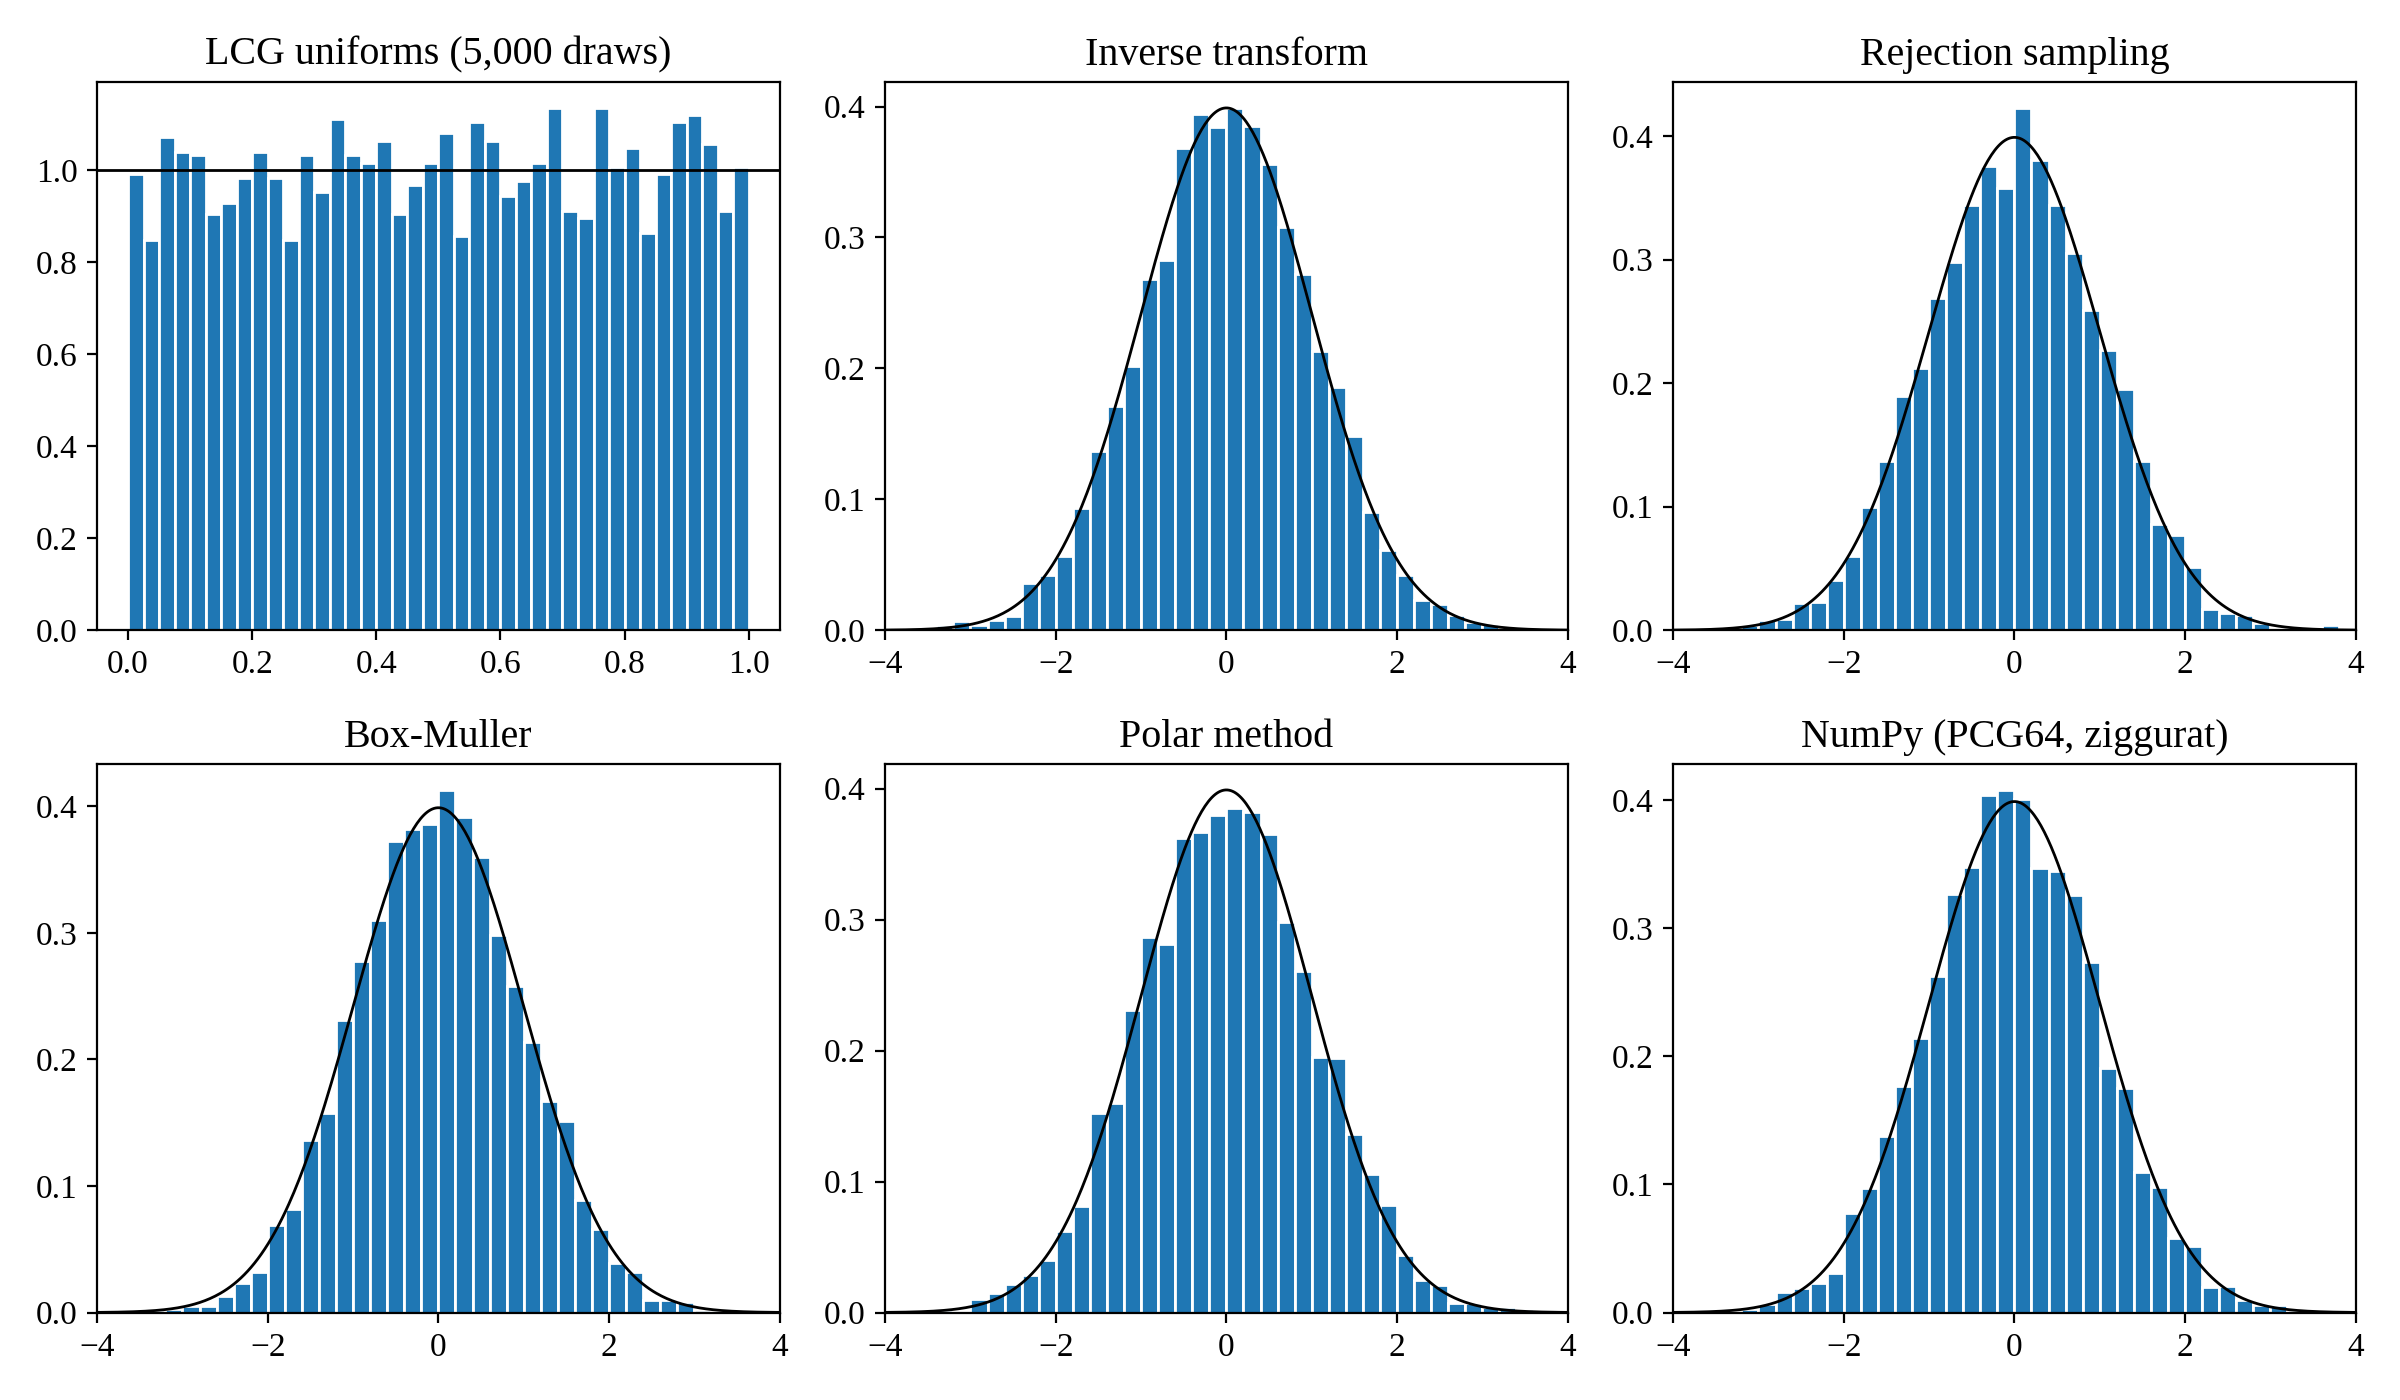
\includegraphics[width=\textwidth]{../figures/histograms.png}
\caption{Histograms of \SampleSize{} draws for each method, with the standard normal density, and of \SampleSize{} LCG uniforms.}
\label{fig:hist}
\end{figure}

\begin{figure}[htbp]
\centering
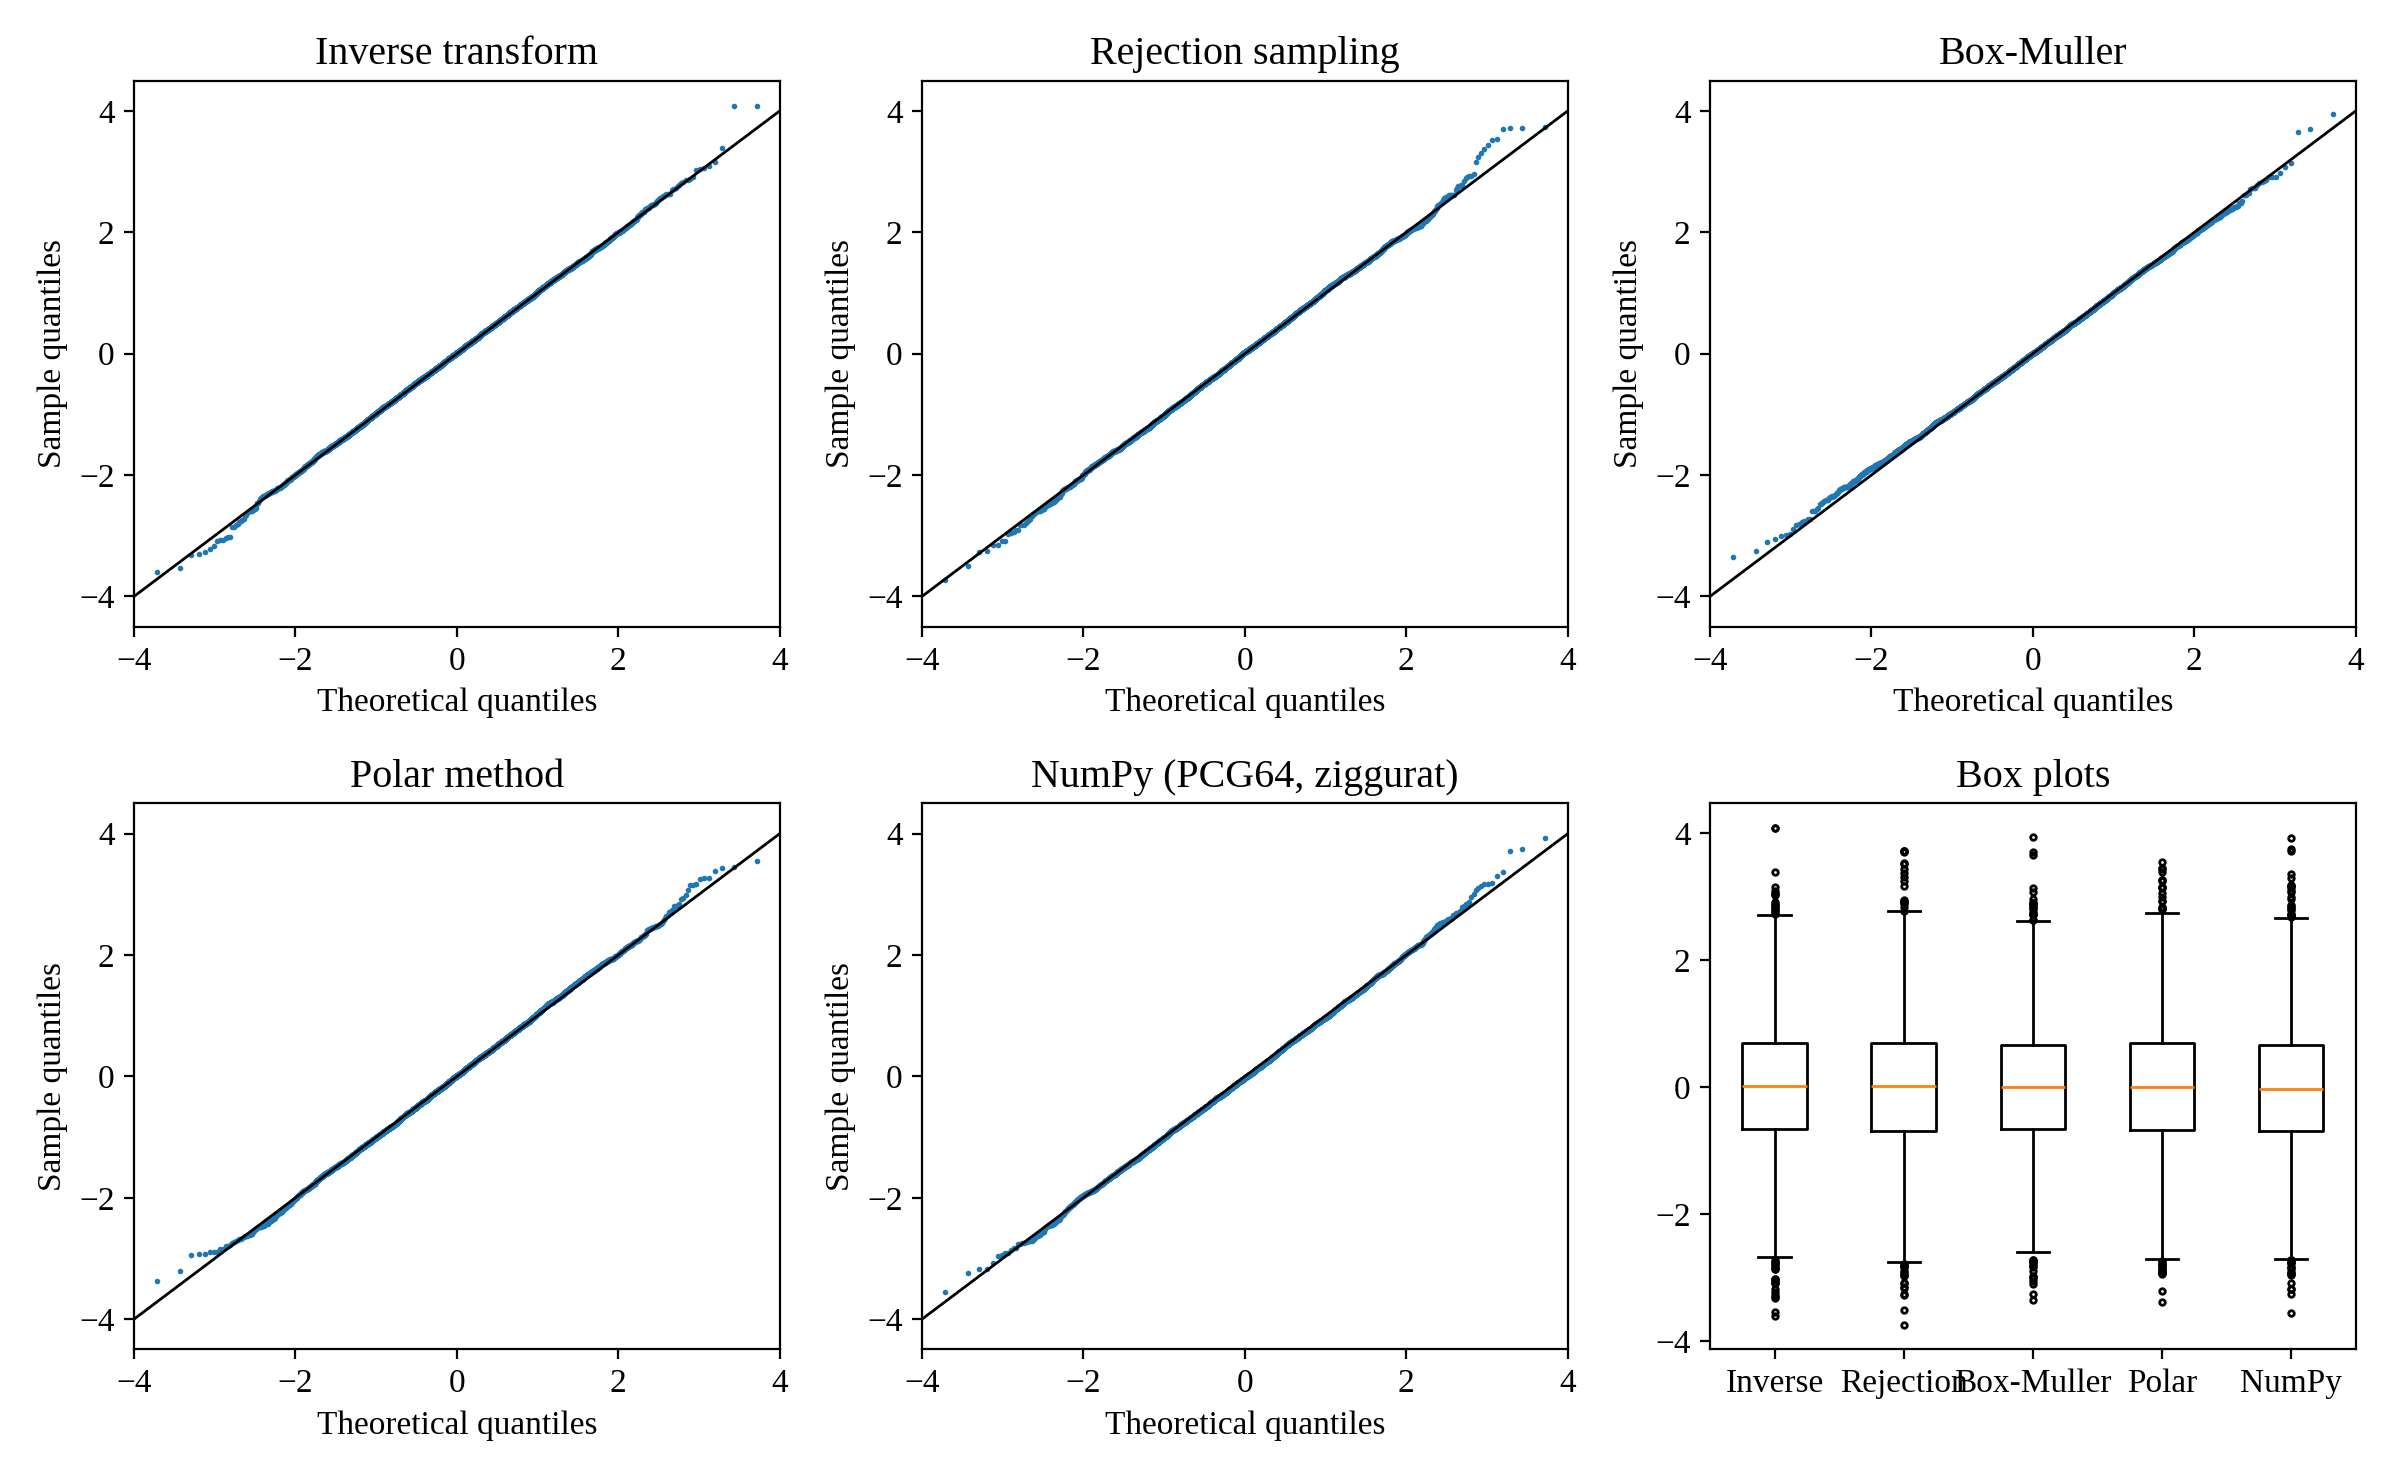
\includegraphics[width=\textwidth]{../figures/qq_plots.png}
\caption{Q-Q plots of the same samples against the standard normal distribution, and box plots of all five samples.}
\label{fig:qq}
\end{figure}

\begin{table}[htbp]
\centering
\caption{Summary statistics and p-values of the normality tests for one sample of \SampleSize{} draws per method.}
\label{tab:single}
\small
\begin{tabular}{lccccc}
\toprule
 & Inverse transform & Rejection & Box-Muller & Polar & NumPy \\
\midrule
Mean & 0.012 & 0.008 & 0.010 & 0.011 & -0.014 \\
Standard deviation & 1.000 & 1.013 & 0.976 & 1.015 & 1.001 \\
Skewness & -0.013 & 0.009 & 0.054 & 0.024 & 0.055 \\
Excess kurtosis & 0.075 & 0.049 & -0.034 & -0.052 & 0.089 \\
\multicolumn{6}{l}{\textit{p-values}} \\
Kolmogorov-Smirnov & 0.726 & 0.453 & 0.344 & 0.453 & 0.280 \\
Anderson-Darling & 0.710 & 0.552 & 0.394 & 0.475 & 0.346 \\
Shapiro-Wilk & 0.786 & 0.190 & 0.471 & 0.479 & 0.378 \\
D'Agostino $K^2$ & 0.512 & 0.733 & 0.265 & 0.609 & 0.123 \\
Jarque-Bera & 0.521 & 0.752 & 0.261 & 0.596 & 0.123 \\
\bottomrule
\end{tabular}

\end{table}

Table~\ref{tab:rejection} repeats the tests on \Reps{} independent samples per method. If the samples are exactly normal, each test should reject in about 5\% of them; with \Reps{} repetitions, the standard error of a rejection rate is \RateSE{} percentage points. All 25 rates lie between \RateMin{} and \RateMax{}, no more than \RateMaxZ{} standard errors from 5\%. At this sample size, the tests cannot distinguish any of the four methods from NumPy's generator.

\begin{table}[htbp]
\centering
\caption{Share of \Reps{} samples of \SampleSize{} draws in which each test rejects normality at the 5\% level.}
\label{tab:rejection}
\small
\begin{tabular}{lccccc}
\toprule
Test & Inverse transform & Rejection & Box-Muller & Polar & NumPy \\
\midrule
Kolmogorov-Smirnov & 3.9\% & 5.9\% & 5.5\% & 5.5\% & 6.1\% \\
Anderson-Darling & 4.6\% & 5.5\% & 5.1\% & 6.3\% & 5.3\% \\
Shapiro-Wilk & 3.6\% & 4.7\% & 5.0\% & 3.8\% & 4.9\% \\
D'Agostino $K^2$ & 4.4\% & 5.6\% & 5.7\% & 4.1\% & 6.2\% \\
Jarque-Bera & 4.4\% & 5.5\% & 5.3\% & 3.8\% & 6.2\% \\
\bottomrule
\end{tabular}

\end{table}

Tests on \SampleSize{} draws say little about the far tails, which matter most for risk measures. We therefore counted the draws with $|Z| > 4$ and $|Z| > 5$ in \TailDraws{} draws per method (Table~\ref{tab:tails}). Under normality, \TailExpFour{} and \TailExpFive{} such draws are expected. All counts are consistent with these numbers: the largest deviation for $|Z| > 4$ is \TailMaxAbsZ{} standard deviations, and the smallest two-sided Poisson p-value for $|Z| > 5$ is \TailMinP{}. In particular, we find no shortage of extreme values for the Box-Muller transformation with our LCG, a known problem when the Box-Muller transformation is combined with some multiplicative congruential generators (Neave, 1973).

\begin{table}[htbp]
\centering
\caption{Number of extreme values in \TailDraws{} draws per method.}
\label{tab:tails}
\small
\begin{tabular}{lccc}
\toprule
Method & $|Z| > 4$ & $|Z| > 5$ & p-value, $|Z| > 5$ \\
\midrule
Inverse transform & 6{,}330 & 71 & 0.09 \\
Rejection & 6{,}336 & 55 & 0.83 \\
Box-Muller & 6{,}372 & 57 & 1.00 \\
Polar & 6{,}399 & 72 & 0.07 \\
NumPy & 6{,}299 & 60 & 0.76 \\
Expected & 6{,}334 & 57.3 &  \\
\bottomrule
\end{tabular}

\end{table}

\subsection{Speed}

Table~\ref{tab:speed} reports how many million normal draws per second each method produces for $10^6$ draws per call (best of seven runs, one thread, \CPU). The uniforms come either from our LCG or from NumPy's PCG64 generator.

\begin{table}[htbp]
\centering
\caption{Million draws per second by uniform source, and average number of uniforms per normal draw.}
\label{tab:speed}
\small
\begin{tabular}{lccc}
\toprule
Method & LCG & PCG64 & Uniforms per draw \\
\midrule
Uniforms only & 216 & 211 &  \\
Inverse transform & 21 & 20 & 1.00 \\
Rejection sampling & 23 & 21 & 3.95 \\
Box-Muller & 34 & 35 & 1.00 \\
Polar method & 42 & 40 & 1.27 \\
NumPy \texttt{standard\_normal} &  & 86 &  \\
\bottomrule
\end{tabular}

\end{table}

The polar method is the fastest of the four (\SpeedPolarLCG{} million draws per second with the LCG). The Box-Muller transformation needs fewer uniforms, but the sine and cosine cost more than the rejection step of the polar method. Inverse transform sampling (\SpeedInvLCG{} million draws per second) pays for the evaluation of the rational approximations, and rejection sampling for its \UniPerDrawRej{} uniforms per draw and the logarithm and exponential in every proposal. The measured acceptance rates are \AccRej{} for rejection sampling (theory: \AccRejTheory) and \AccPolar{} for the polar method (theory: \AccPolarTheory). NumPy's ziggurat method, implemented in compiled code, produces \SpeedNumpy{} million draws per second. The choice of uniform generator matters little, since the uniforms are only a small part of the cost.

The ranking depends on the implementation. In a loop that generates one number at a time, the overhead of the interpreter dominates, and methods with a rejection loop look much slower than they are.

% ---------------------------------------------------------------------------------
\section{Monte Carlo Simulation}

Using the inverse transformation sampling method, we can now perform a Monte Carlo simulation to compute the VaR and the ES for a portfolio of two ETFs. The portfolio holds EUR 1.5 million in an ETF on the S\&P 500 and EUR 1.0 million in an ETF on the FTSE 100. Its value in EUR depends on four risk factors: the returns of the two indices and the changes of the USD/EUR and GBP/EUR exchange rates. We model the daily returns $r$ of the four risk factors as multivariate normal, $r \sim N(\mu, \Sigma)$, with the mean vector $\mu$ and covariance matrix $\Sigma$ estimated from 245 daily returns.

We start by generating independent standard normal draws $z$. Each scenario needs four of these, one per factor; we draw the underlying uniforms from NumPy's PCG64 generator rather than the LCG, since the output of an LCG lies on a limited number of hyperplanes in higher dimensions (Marsaglia, 1968) and would bias a four-dimensional simulation. Thereafter, we use the Cholesky decomposition of the covariance matrix $\Sigma$ to obtain correlated returns. The Cholesky decomposition of $\Sigma$ is a decomposition of the form
\[
\Sigma = L L^{T},
\]
where $L$ is a lower triangular matrix with real and positive diagonal entries, and $L^{T}$ denotes the transpose of $L$.\footnote{The decomposition exists if $\Sigma$ is positive definite.} Correlated returns can then be obtained by
\[
r = \mu + L z,
\]
since $\mathrm{Cov}(Lz) = L\,I\,L^{T} = \Sigma$.\footnote{For example, for two standardised returns with correlation $\rho$, $L = \begin{bmatrix} 1 & 0 \\ \rho & \sqrt{1-\rho^2}\end{bmatrix}$.} The one-day change in the value of the portfolio is
\[
\Delta V = 1.5\,\text{m}\,(1 + r_{\text{S\&P}})(1 + r_{\text{USD}}) + 1.0\,\text{m}\,(1 + r_{\text{FTSE}})(1 + r_{\text{GBP}}) - 2.5\,\text{m}.
\]
Finally, we can calculate our desired risk measures, which can be defined as follows:

\textbf{VaR:} For a position $V$ with random changes in value $\Delta V$ over a time horizon $[0, \Delta t]$, the VaR at the confidence level $\alpha \in (0,1)$ is given by the smallest number $l$ such that the probability that the loss $-\Delta V$ exceeds $l$ is no larger than $1 - \alpha$.

\textbf{ES:} For a position $V$ with random changes in value $\Delta V$ over a time horizon $[0, \Delta t]$, the ES at the confidence level $\alpha \in (0,1)$ is the expected value of the loss, given that the loss exceeds $\text{VaR}_\alpha$.

With $n$ simulated scenarios sorted as $\Delta V_{(1)} \le \dots \le \Delta V_{(n)}$ and $k = \lfloor (1-\alpha) n + 1 \rfloor$, we estimate the VaR as $-\Delta V_{(k)}$ and the ES as minus the average of the $(1-\alpha)n$ worst scenarios. If $(1-\alpha)n$ is not an integer, the $k$-th scenario enters the average with the weight $1 + (1-\alpha)n - k$. We use $\alpha = 99\%$.

Table~\ref{tab:var} summarises the results. With \RefDraws{} scenarios, the one-day 99\% VaR is EUR \VaRRef{} and the ES is EUR \ESRef. The delta-normal approximation, which drops the products of index and exchange-rate returns so that $\Delta V$ is exactly normal, gives similar values (EUR \VaRDN{} and \ESDN).

\begin{table}[htbp]
\centering
\caption{One-day 99\% VaR and ES of the portfolio.}
\label{tab:var}
\small
\begin{tabular}{lcc}
\toprule
 & VaR (EUR) & ES (EUR) \\
\midrule
Monte Carlo, the spreadsheet's 500 draws & 78{,}329 & 85{,}175 \\
Monte Carlo, 500 draws, 5\% to 95\% range over 500 runs & 69{,}936 to 87{,}738 & 79{,}328 to 100{,}870 \\
Monte Carlo, 10 million draws & 79{,}166 & 90{,}413 \\
Delta-normal (linearised value change) & 79{,}689 & 91{,}165 \\
\bottomrule
\end{tabular}

\end{table}

An earlier spreadsheet version of this example used 500 scenarios. Given the same 500 normal draws, our code reproduces the spreadsheet's VaR of EUR \VaRSheet{} exactly. The spreadsheet's ES of EUR \ESSheetReported{} was computed from a sorted copy of the scenarios that had not been updated after the last recalculation; with the same draws, the ES is EUR \ESSheet.

Figure~\ref{fig:var} shows the distribution of the simulated value changes and how the VaR estimate depends on the number of scenarios. With 500 scenarios, the estimates vary with a standard deviation of EUR \VaRSDFiveHundred{} across \ConvReps{} repetitions, about \VaRSDPct\% of the VaR, and 90\% of them lie between EUR \VaRLoFiveHundred{} and \VaRHiFiveHundred. The spreadsheet's value lies at the \VaRRankSheet{}th percentile of these estimates, so it was a typical outcome. The estimator is also slightly biased downwards in small samples: with 500 scenarios its average is \VaRBiasPct\% below the value with \RefDraws{} draws. The standard deviation falls with roughly $1/\sqrt{n}$, to EUR \VaRSDTenK{} for 10{,}000 scenarios and EUR \VaRSDHundredK{} for 100{,}000. For a risk figure that should not move much from one day to the next for purely numerical reasons, 500 scenarios are too few.

\begin{figure}[htbp]
\centering
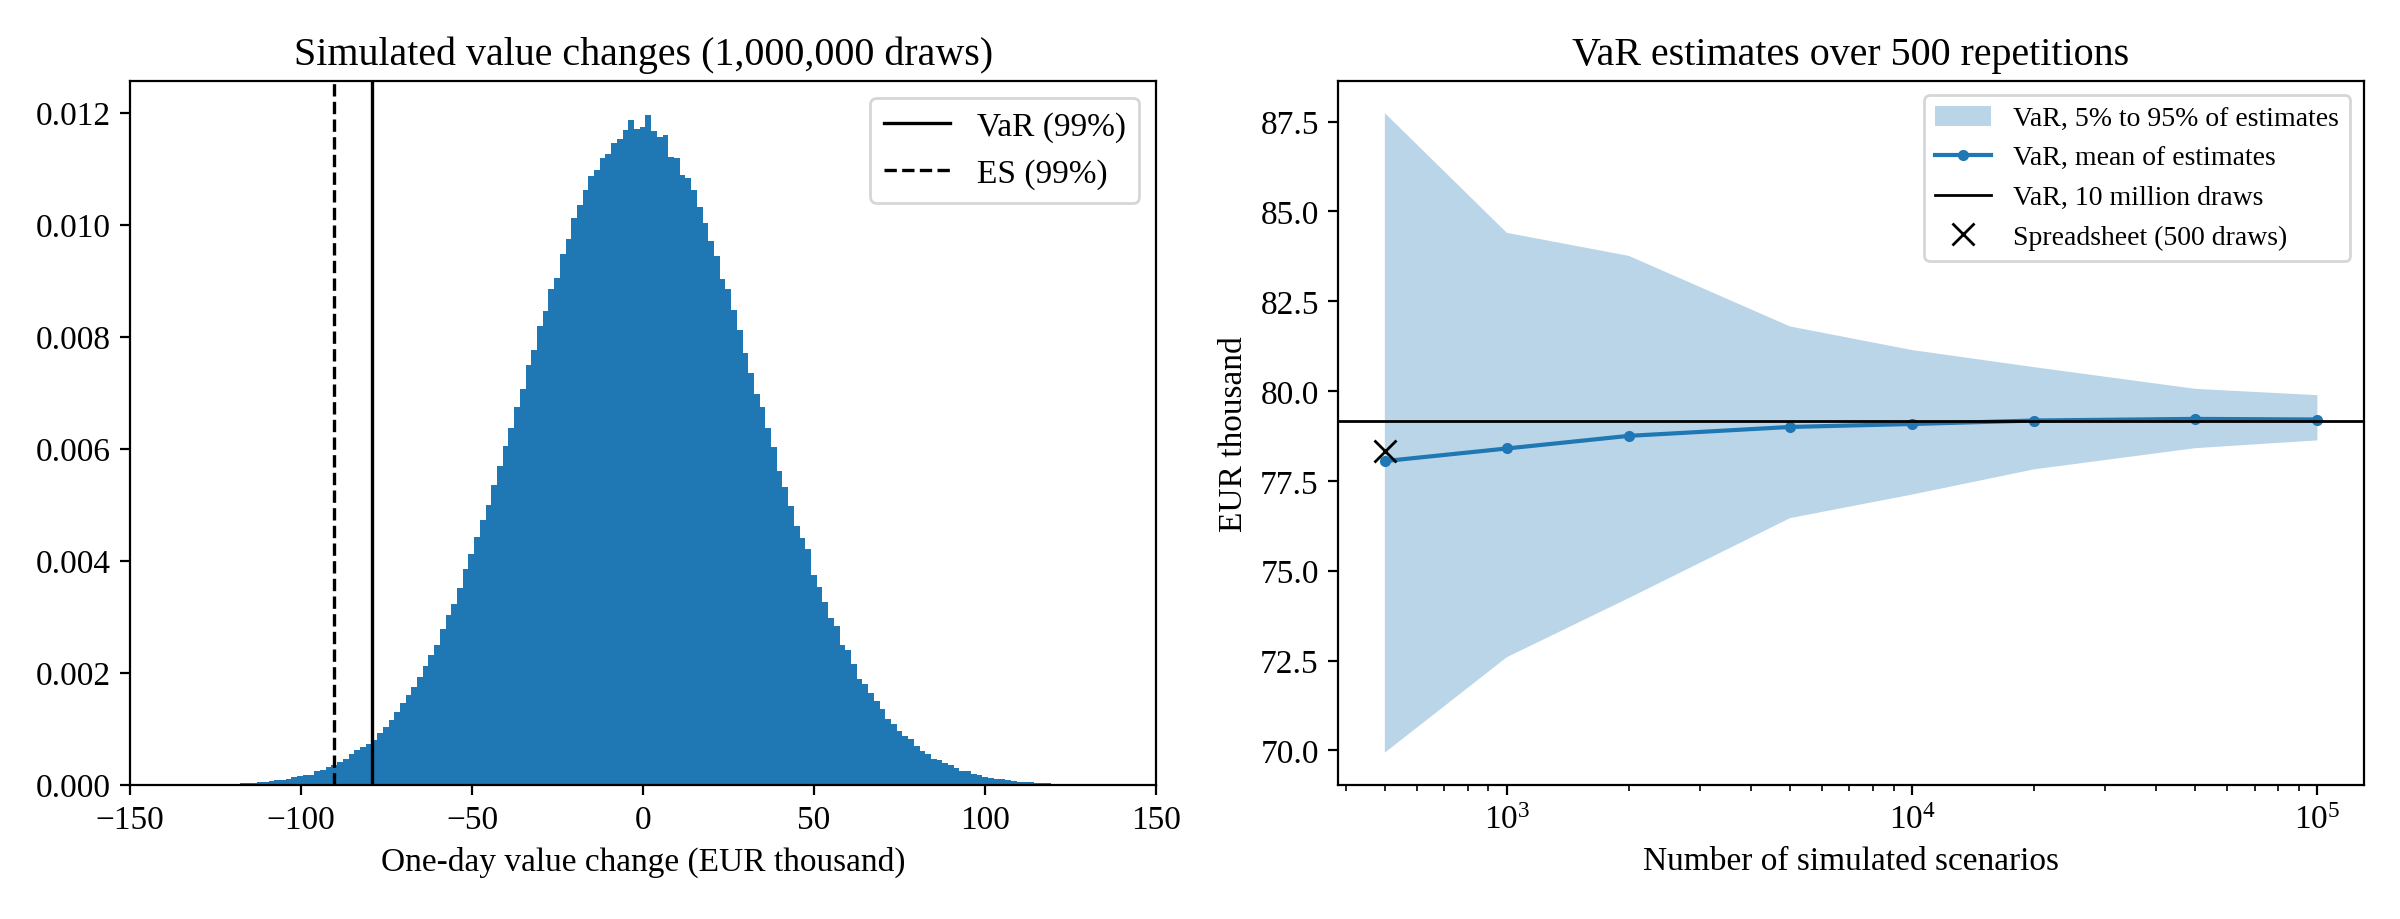
\includegraphics[width=\textwidth]{../figures/var.png}
\caption{Left: one-day value changes in one million scenarios, with the 99\% VaR and ES. Right: mean and 5\% to 95\% range of the VaR estimates over \ConvReps{} repetitions, by number of scenarios.}
\label{fig:var}
\end{figure}

% ---------------------------------------------------------------------------------
\section{Conclusion}

All four methods turn the output of a simple LCG into samples that pass the standard normality tests at their nominal rate, also when the tests are repeated many times, and that contain the expected number of extreme values in \TailDraws{} draws. The methods differ mainly in speed and simplicity. The polar method was the fastest in our vectorised implementation. Inverse transform sampling is slower, but it needs exactly one uniform per draw and is monotone in $u$, which makes it the natural choice for variance reduction techniques such as antithetic variates and for quasi-random sequences.

In the VaR example, the main source of error is not the normal generator but the number of scenarios: with 500 scenarios, the 99\% VaR has a standard error of about \VaRSDPct\%.

% ---------------------------------------------------------------------------------
\clearpage
\section*{References}
\begin{list}{}{\leftmargin=0pt\itemsep=6pt\parsep=0pt}
\item[] [1] Anderson, T.W. \& Darling, D.A. (1952), `Asymptotic theory of certain goodness-of-fit criteria based on stochastic processes', in: The Annals of Mathematical Statistics, Vol. 23, No. 2, pp. 193-212.
\item[] [2] Bera, A.K. \& Jarque, C.M. (1982), `Model specification tests: A simultaneous approach', in: Journal of Econometrics, Vol. 20, pp. 59-82.
\item[] [3] Box, G.E.P. \& Muller, M.E. (1958), `A note on the generation of random normal deviates', in: The Annals of Mathematical Statistics, Vol. 29, No. 2, pp. 610-611.
\item[] [4] D'Agostino, R.B. (1971), `An omnibus test of normality for moderate and large sample sizes', in: Biometrika, Vol. 58, No. 2, pp. 341-348.
\item[] [5] D'Agostino, R.B. (1986), `Tests for normal distribution', in: Goodness-of-fit Techniques, edited by D'Agostino, R.B. and Stephens, M.A., pp. 367-420, Marcel Dekker, New York.
\item[] [6] D'Agostino, R.B. \& Pearson, E.S. (1973), `Tests for departure from normality. Empirical results for the distributions of $b_2$ and $\sqrt{b_1}$', in: Biometrika, Vol. 60, No. 3, pp. 613-622.
\item[] [7] Devroye, L. (1986), `Non-uniform Random Variate Generation', Springer-Verlag, New York.
\item[] [8] Hull, T.E. \& Dobell, A.R. (1962), `Random number generators', in: SIAM Review, Vol. 4, No. 3, pp. 230-254.
\item[] [9] Knuth, D.E. (1997), `The Art of Computer Programming, Vol. 2: Seminumerical Algorithms', 3rd edition, Addison-Wesley, Reading.
\item[] [10] Kolmogorov, A. (1933), `Sulla determinazione empirica di una legge di distribuzione', in: Giornale dell'Istituto Italiano degli Attuari, Vol. 4, pp. 83-91.
\item[] [11] Lilliefors, H.W. (1967), `On the Kolmogorov-Smirnov test for normality with mean and variance unknown', in: Journal of the American Statistical Association, Vol. 62, No. 318, pp. 399-402.
\item[] [12] Marsaglia, G. (1968), `Random numbers fall mainly in the planes', in: Proceedings of the National Academy of Sciences, Vol. 61, No. 1, pp. 25-28.
\item[] [13] Marsaglia, G. \& Bray, T.A. (1964), `A convenient method for generating normal variables', in: SIAM Review, Vol. 6, No. 3, pp. 260-264.
\item[] [14] Marsaglia, G. \& Marsaglia, J. (2004), `Evaluating the Anderson-Darling distribution', in: Journal of Statistical Software, Vol. 9, No. 2, pp. 1-5.
\item[] [15] Marsaglia, G. \& Tsang, W.W. (2000), `The ziggurat method for generating random variables', in: Journal of Statistical Software, Vol. 5, No. 8, pp. 1-7.
\item[] [16] Murison, M.A. (2000), `A method for directly generating a Gaussian distribution with nonunit variance and nonzero mean from uniform random deviates', Washington.
\item[] [17] Neave, H.R. (1973), `On using the Box-Muller transformation with multiplicative congruential pseudo-random number generators', in: Applied Statistics, Vol. 22, No. 1, pp. 92-97.
\item[] [18] O'Neill, M.E. (2014), `PCG: A family of simple fast space-efficient statistically good algorithms for random number generation', Technical Report HMC-CS-2014-0905, Harvey Mudd College.
\item[] [19] Shapiro, S.S. \& Wilk, M.B. (1965), `An analysis of variance test for normality (complete samples)', in: Biometrika, Vol. 52, No. 3/4, pp. 591-611.
\item[] [20] Sigman, K. (2007), `Acceptance-rejection method', lecture notes, Columbia University.
\item[] [21] Smirnov, N. (1948), `Table for estimating the goodness of fit of empirical distributions', in: The Annals of Mathematical Statistics, Vol. 19, No. 2, pp. 279-281.
\item[] [22] Wichura, M.J. (1988), `Algorithm AS 241: The percentage points of the normal distribution', in: Applied Statistics, Vol. 37, No. 3, pp. 477-484.
\end{list}

\section*{GitHub Repository}
\url{https://github.com/duemig/normal-random-number-generation}

% ---------------------------------------------------------------------------------
\clearpage
{\appendixfont
\setcounter{section}{0}
\renewcommand{\thesection}{\Roman{section}.}
\titleformat{\section}{\fontsize{16}{19}\selectfont\bfseries}{\thesection}{0.6em}{}

{\fontsize{16}{19}\selectfont\bfseries Appendix\par}
\vspace{4pt}

\section{Proofs of the Inverse Sampling Algorithm}

\textbf{Proof of Case 1.} We first notice the following facts:
\begin{itemize}
\item $x \le y \Rightarrow F(x) \le F(y)$, because $F$ is a CDF and a CDF is non-decreasing.
\item $x < y \Rightarrow F(x) < F(y)$: since $F$ is invertible, $F(x) \ne F(y)$ for $x \ne y$, and combining this with the previous statement gives $F(x) < F(y)$.
\item $a \le b \Rightarrow F^{-1}(a) \le F^{-1}(b)$ for $a, b \in (0,1)$. We prove this by contradiction. Suppose $a \le b$ and $F^{-1}(a) > F^{-1}(b)$. Then, by the previous statement, $a = F(F^{-1}(a)) > F(F^{-1}(b)) = b$, which is a contradiction.
\end{itemize}
Now let $U \sim \text{Uniform}(0,1)$ and let $H$ denote the CDF of the uniform distribution,
\[
H(x) = \begin{cases} 0, & x \le 0,\\ x, & 0 < x < 1,\\ 1, & x \ge 1.\end{cases}
\]
By the second and third fact, $F^{-1}(U) \le x$ holds if and only if $U \le F(x)$. Hence
\[
P\left(F^{-1}(U) \le x\right) = P\left(U \le F(x)\right) = H\left(F(x)\right) = F(x),
\]
as the range of $F$ is $(0,1)$. This implies $F^{-1}(U) \sim F$. \hfill$\square$

\textbf{Proof of Case 2.} First, we notice that if $F$ is invertible, then $G = F^{-1}$, and that $G(a)$ is a finite real number for $a \in (0,1)$, since $F(x) \to 1$ as $x \to \infty$ and $F(x) \to 0$ as $x \to -\infty$. We now prove the following claim.

\textbf{Claim:} For all $a \in (0,1)$ and $y \in \mathbb{R}$: $a \le F(y)$ if and only if $G(a) \le y$.

\textbf{Proof:} Suppose $a \le F(y)$. Then $y \in \{x: a \le F(x)\}$, so $y \ge \inf\{x: a \le F(x)\} = G(a)$. To prove the converse, we prove the contrapositive statement, i.e.\ that $a > F(y)$ implies $G(a) > y$. So assume $a > F(y)$. By right continuity of $F$, there is $y_0 > y$ such that $F(y_0) < a$. Since $F$ is non-decreasing, $F(x) \le F(y_0) < a$ for all $x \le y_0$, so $\{x: a \le F(x)\} \subset (y_0, \infty)$ and $G(a) \ge y_0 > y$.

With the claim, repeating the last argument of the proof of Case 1 gives
\[
P\left(G(U) \le x\right) = P\left(U \le F(x)\right) = H\left(F(x)\right) = F(x).
\]
Hence $G(U) \sim F$. \hfill$\square$

\section{Acceptance-Rejection Algorithm}

\begin{enumerate}
\item Generate a random variable $Y$ with density $g$.
\item Generate $U \sim \text{Uniform}(0,1)$, independent of $Y$.
\item If $U \le \dfrac{f(Y)}{c\,g(Y)}$, set $X = Y$ (``accept''); otherwise go back to 1 (``reject'').
\end{enumerate}

Before proving that this works, we notice the following:
\begin{itemize}
\item $f(Y)$ and $g(Y)$ are random variables, and so is the ratio $\dfrac{f(Y)}{c\,g(Y)}$. This ratio is independent of $U$ in step 2, and it lies between 0 and 1.
\item The number $N$ of times steps 1 and 2 have to be carried out until $X$ is generated is itself a random variable. It has a geometric distribution with ``success'' probability $p = P\left(U \le \frac{f(Y)}{c\,g(Y)}\right)$: $P(N = n) = (1-p)^{n-1}p$, $n \ge 1$. Thus, on average the number of iterations required is $E(N) = 1/p$.
\item In the end, $X$ has the conditional distribution of $Y$ given that the event $\left\{U \le \frac{f(Y)}{c\,g(Y)}\right\}$ occurs.
\end{itemize}

A direct calculation yields $p = 1/c$. Conditioning on $Y$ gives $P\left(U \le \frac{f(Y)}{c\,g(Y)} \,\middle|\, Y = y\right) = \frac{f(y)}{c\,g(y)}$; unconditioning and recalling that $Y$ has density $g$ yields
\[
p = \int_{-\infty}^{\infty} \frac{f(y)}{c\,g(y)}\, g(y)\,dy = \frac{1}{c}\int_{-\infty}^{\infty} f(y)\,dy = \frac{1}{c},
\]
where the last equality follows since $f$ is a density and integrates to 1. Thus $E(N) = c$, the bounding constant, and it is desirable to choose the alternative density $g$ so as to minimise $c = \sup_x \{f(x)/g(x)\}$. The optimal choice would be $g = f$, which is not what we have in mind, since the whole point is to sample from a different density. For the half-normal density and the exponential proposal of Section 2.3, $c = \sqrt{2e/\pi} \approx 1.32$.

\textbf{Proof that the algorithm works.} We must show that the conditional distribution of $Y$, given that $U \le \frac{f(Y)}{c\,g(Y)}$, is $F$, i.e.\ that $P\left(Y \le y \,\middle|\, U \le \frac{f(Y)}{c\,g(Y)}\right) = F(y)$. Let $B = \left\{U \le \frac{f(Y)}{c\,g(Y)}\right\}$ and $A = \{Y \le y\}$, and let $G$ be the CDF of $Y$. Recalling that $P(B) = 1/c$ and using $P(A \mid B) = P(B \mid A)\,P(A)/P(B)$ yields
\[
P(A \mid B) = \frac{F(y)}{c\,G(y)} \times \frac{G(y)}{1/c} = F(y),
\]
where we used the following computation:
\[
P(B \mid A) = \frac{P\left(U \le \frac{f(Y)}{c\,g(Y)},\, Y \le y\right)}{G(y)}
= \frac{1}{G(y)}\int_{-\infty}^{y} \frac{f(w)}{c\,g(w)}\, g(w)\,dw
= \frac{1}{c\,G(y)}\int_{-\infty}^{y} f(w)\,dw = \frac{F(y)}{c\,G(y)}.
\]
\hfill$\square$

\section{Proof of the Box-Muller Transformation}

Let $u_1, u_2$ be independent and uniform on $(0,1)$, and let $z_1 = R\cos\theta$, $z_2 = R\sin\theta$ with $R = \sqrt{-2\ln u_1}$ and $\theta = 2\pi u_2$. The map $(u_1, u_2) \mapsto (z_1, z_2)$ is one-to-one, with inverse
\[
u_1 = \exp\left(-\frac{z_1^2 + z_2^2}{2}\right), \qquad u_2 = \frac{1}{2\pi}\arctan\left(\frac{z_2}{z_1}\right) \ (\text{taken in the correct quadrant}).
\]
The fundamental transformation law of probabilities states that $|p(y)\,dy| = |p(x)\,dx|$, or $p(y) = p(x)\left|\frac{dx}{dy}\right|$. Its extension to $n$ dimensions is $p(y_1, \dots, y_n) = p(x_1, \dots, x_n)\,|J|$, where $J$ is the Jacobi determinant of the map from $(y_1, \dots, y_n)$ to $(x_1, \dots, x_n)$. Here $p(u_1, u_2) = 1$ and
\[
J = \det\begin{bmatrix} \dfrac{\partial u_1}{\partial z_1} & \dfrac{\partial u_1}{\partial z_2} \\[8pt] \dfrac{\partial u_2}{\partial z_1} & \dfrac{\partial u_2}{\partial z_2}\end{bmatrix}
= \det\begin{bmatrix} -z_1 u_1 & -z_2 u_1 \\[4pt] -\dfrac{z_2}{2\pi(z_1^2 + z_2^2)} & \dfrac{z_1}{2\pi(z_1^2 + z_2^2)}\end{bmatrix}
= -\frac{u_1}{2\pi}.
\]
Hence
\[
p(z_1, z_2) = \frac{1}{2\pi}\exp\left(-\frac{z_1^2 + z_2^2}{2}\right) = \frac{1}{\sqrt{2\pi}}e^{-z_1^2/2} \cdot \frac{1}{\sqrt{2\pi}}e^{-z_2^2/2},
\]
so $z_1$ and $z_2$ are independent standard normal random variables. For $x_i = \mu + \sigma z_i$, the Jacobi determinant of the linear map is $1/\sigma^2$, and
\[
p(x_1, x_2) = \frac{1}{2\pi\sigma^2}\exp\left(-\frac{(x_1-\mu)^2 + (x_2-\mu)^2}{2\sigma^2}\right),
\]
i.e.\ $(x_1, x_2)$ has a symmetric bivariate Gaussian distribution with independent components, mean $\mu$ and variance $\sigma^2$. \hfill$\square$

\section{Proof of the Polar Method}

After the rejection step, $(V_1, V_2)$ is uniform on the unit disc with density $1/\pi$. In polar coordinates, $V_1 = R\cos\theta$ and $V_2 = R\sin\theta$, and the Jacobi determinant of the map is $r$, so $(R, \theta)$ has the density $r/\pi$ on $(0,1) \times (0, 2\pi)$. This density factorises: $\theta$ is uniform on $(0, 2\pi)$ and independent of $R$, and
\[
P(R^2 \le s) = \int_0^{\sqrt{s}} 2r\,dr = s, \qquad 0 < s < 1,
\]
so $S = R^2$ is uniform on $(0,1)$. With $u_1 = S$ and $u_2 = \theta/(2\pi)$, which are independent and uniform on $(0,1)$, the Box-Muller formulas give
\[
z_1 = \sqrt{-2\ln S}\cos\theta = V_1\sqrt{\frac{-2\ln S}{S}}, \qquad z_2 = \sqrt{-2\ln S}\sin\theta = V_2\sqrt{\frac{-2\ln S}{S}},
\]
which are independent standard normal random variables by Appendix III. \hfill$\square$
}

\end{document}
